\chapter{Results}
\label{ch:results}
The Kalman filter and controls algorithms discussed in this thesis were implemented in software on a Packbot and run in an open field with an uneven surface consisting of dirt, gravel and asphalt as seen in Figure \ref{fig:resultsTestArea}. This testing area is difficult for the robots to navigate because pitch, roll and elevation have significant changes and the loose dirt and gravel can cause the tracks to slip leading to erroneous encoder data. The environment in addition to routes that force the robot to change linear and angular velocities excites all the modes of the system model as well as some effects, such as track slip, which are not modeled at all and rigorously tests the estimation and control algorithms.

\begin{figure}[ht!]
	\centering
	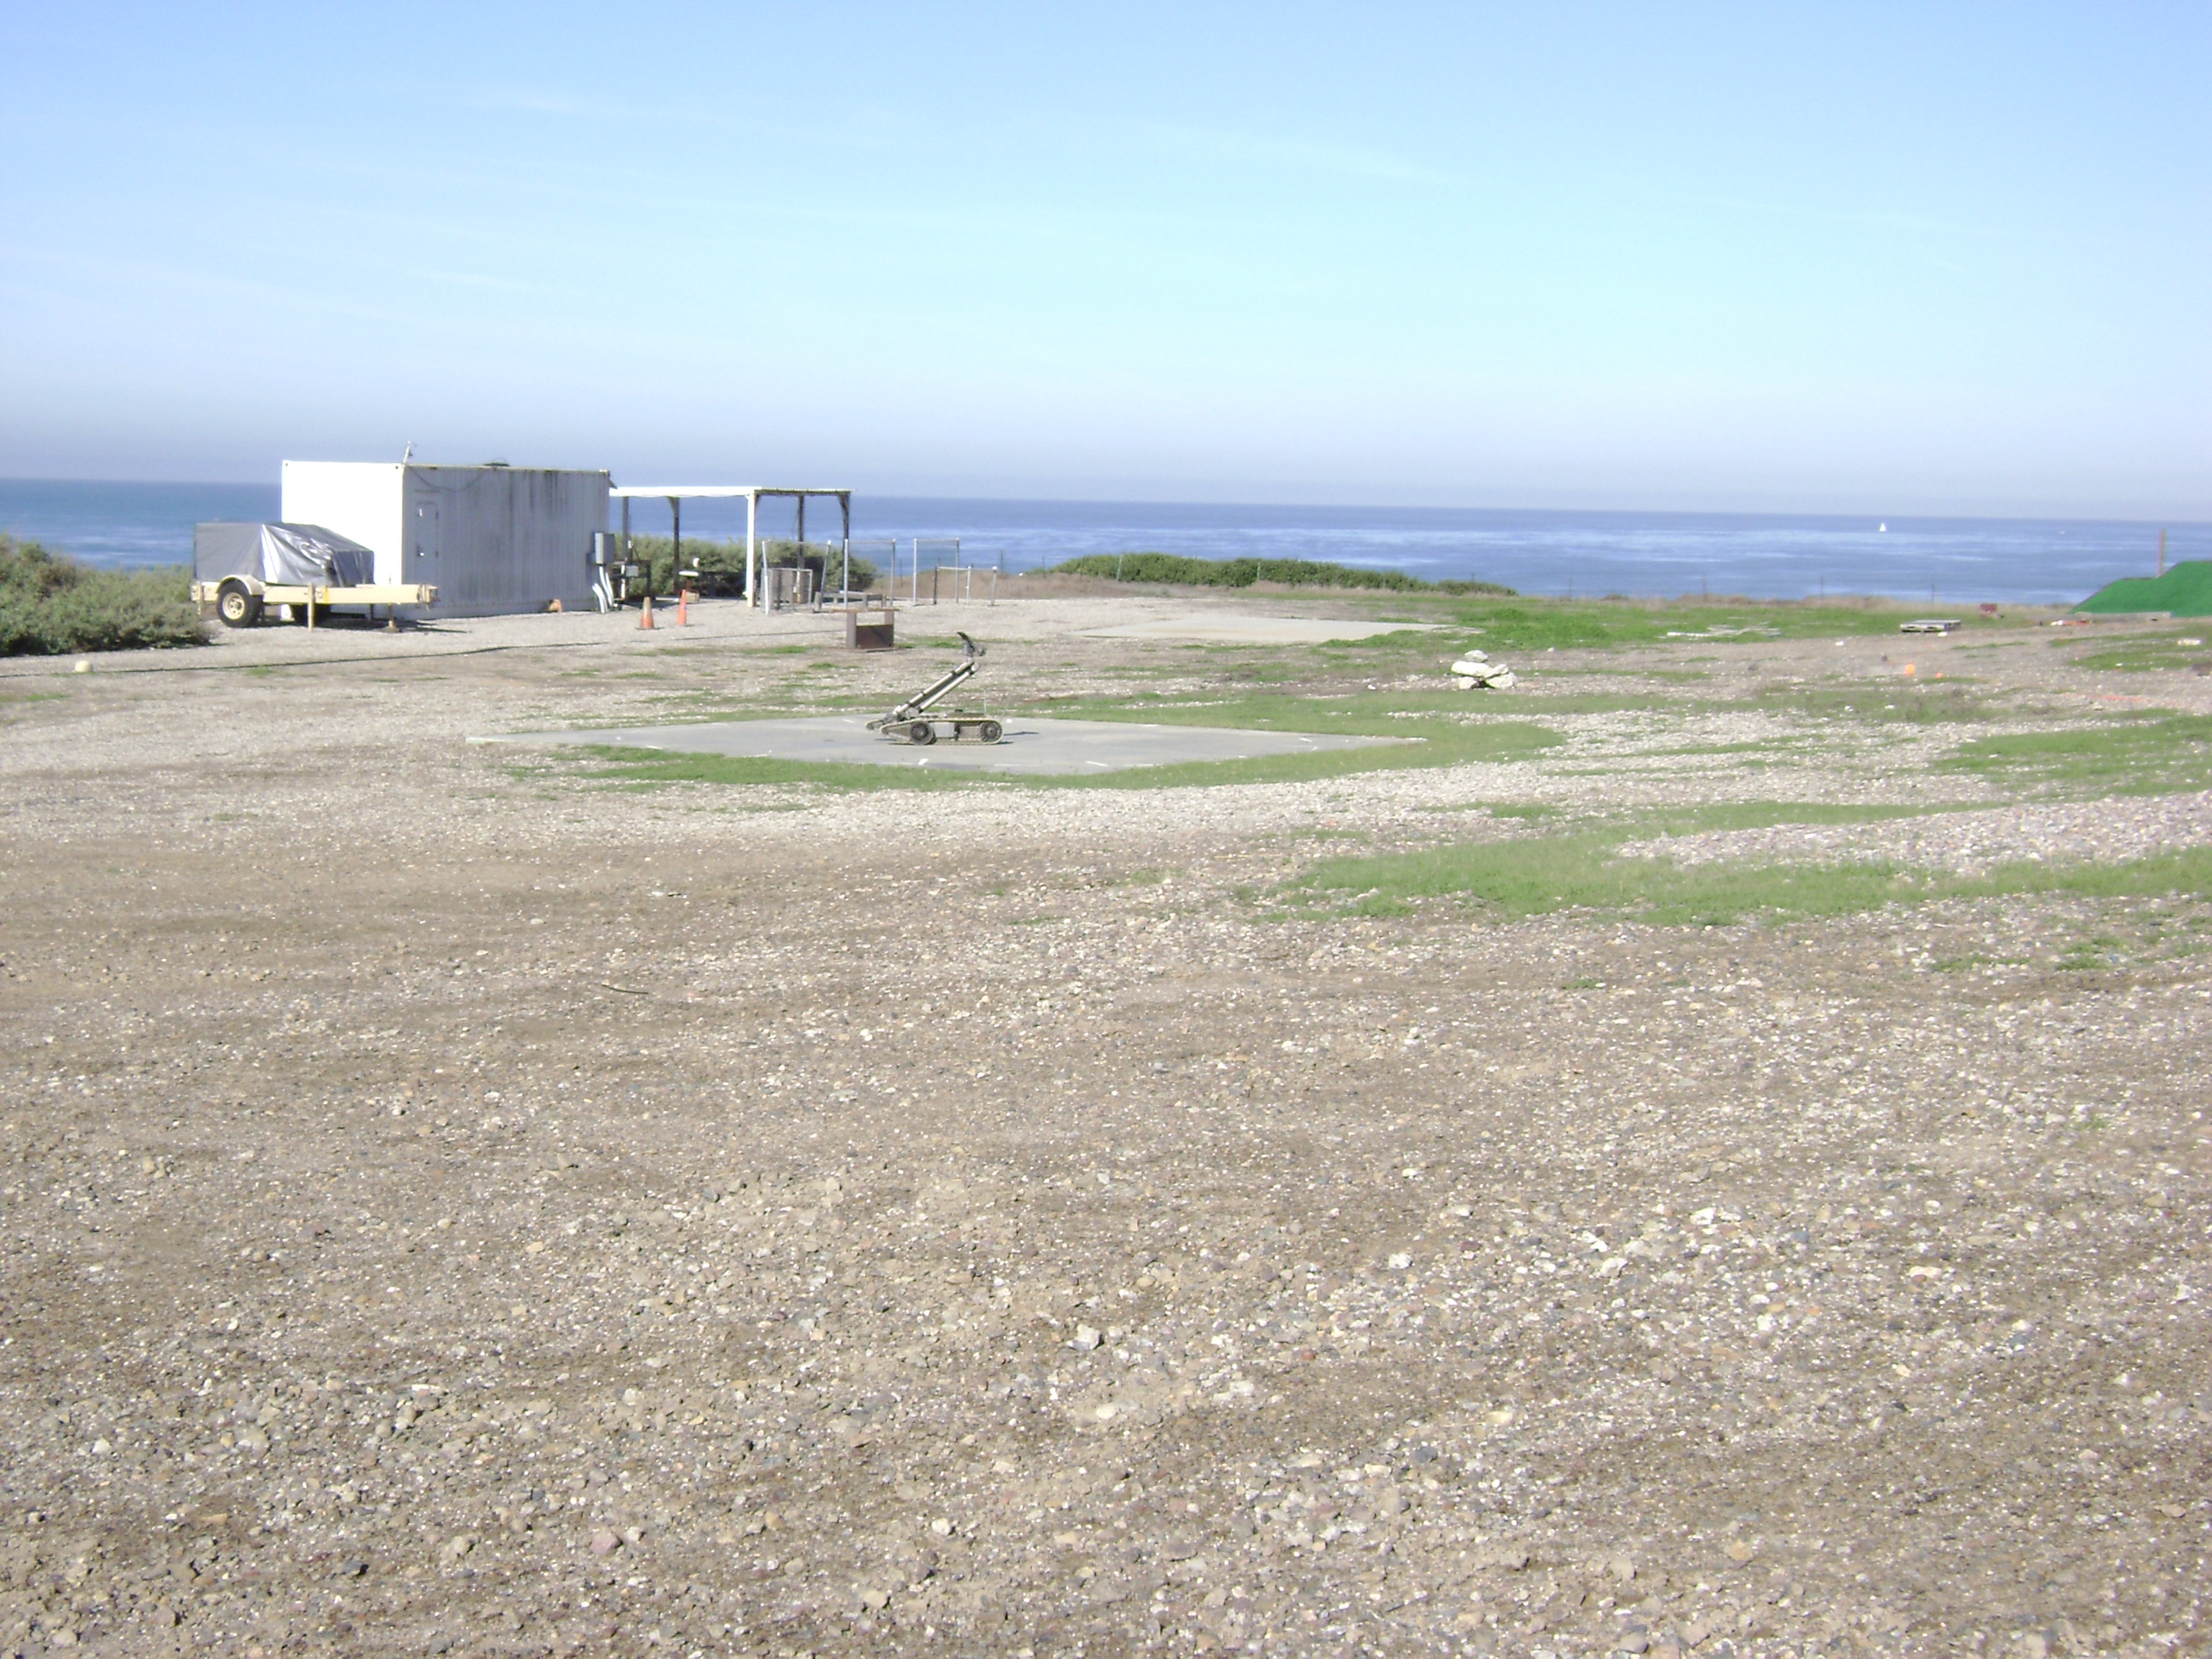
\includegraphics[width=.75\textwidth]{images/flightFieldTestArea}
	\caption{Robot Test Area}
	\label{fig:resultsTestArea}
\end{figure}

\section{Kalman Filter Results}
\label{sec:kfResults}
In Chapter \ref{ch:estimation} several aspects of the Kalman filter were modified with the goal of improving robot state estimation. Two metrics have been used to quantify the difference in performance of the Kalman filter after having made changes to the algorithm. Those metrics are the RMS error over the entire course and the amount of error in the position estimate before and after the robot runs a route where the percentage is the position error divided by the total amount of distance traveled over the route. Also included is the total distance traveled during the run that the data was logged. The different changes that were tested were the baseline case, fixing the Kalman filter implementation bugs described in Chapter \ref{sec:kfBugs}, hand tuning the Kalman filter noise models and finally using noise models learned from the training algorithm from Chapter \ref{sec:kftrainingparams}. The results for Kalman filter performance are shown in Table \ref{tab:resultsKF}.

% Note for data sources: baseline is 20010107_1037, fixes is 20100107_1411, hand tuned is 20100107_1415, trained is 20100107_1905.
\begin{table}[ht!]
\caption{Kalman Filter Performance}
\small
\centering
\begin{tabular}{@{}lllr@{}} \toprule
Stage      & RMS Error (m)  & Return Error (\%) & Distance Traveled (m) \\ \midrule
Baseline   & 10.62          & 1.51              & 224.22 \\
Fix Bugs   & 4.38           & 0.79              & 182.70 \\
Hand Tuned & 4.87           & 1.32              & 184.09 \\
Trained    & 3.64           & 0.99              & 332.62 \\ \bottomrule
\end{tabular}
\label{tab:resultsKF}
\end{table}

The most significant improvement came from fixing the bugs in the Kalman filter code. Using the training algorithm to tune the parameters in the noise models showed a marked improvement over the hand tuned case and was also better on average than the case where the bugs were fixed. Although the trained noise models case has a slightly greater error in the difference between starting and stopping positions that run was much greater in total distance traveled and a return error of $0.99\%$ over a $332m$ run is more than sufficient to perform retrotraverse in most environments where the robots are used.

\subsection{Kalman Filter Effects on Controller}
Early on during testing, before the bugs were discovered and fixed in the Kalman filter, several runs were logged that show how estimation errors can affect the model based and PID controllers. In this section the data was collected before the bugs in the Kalman filter were fixed (Chapter \ref{sec:kfBugs}) but training of the noise models was used (Chapter \ref{sec:kftrainingparams}). The results are interesting because they show that the previous performance of the PID controller could break down and become unusable as well as because it shows that the training algorithm can improve a filter with equations that are not optimal. The results show that not only is the Kalman filter performance better after using the training algorithm but it can also be seen that the model based controller has much better performance when there are simulated obstacles along the route.

In Figures \ref{fig:kfResults1} - \ref{fig:kfResults4} the same route was driven and the waypoints making up the route are shown on the overhead images. The red line is the Kalman filter position esimate, the blue line is raw GPS measurements and the green line is DPGS measurements.

The results of using the model based controller with original noise models is shown in Figure \ref{fig:kfResults1}. It can be seen that going from waypoint $4$ to waypoint $5$ the Kalman filter started to diverge significantly from the GPS measurements and the filter estimate snaps back to line up with the GPS measurements.

\begin{figure}[ht!]
	\centering
	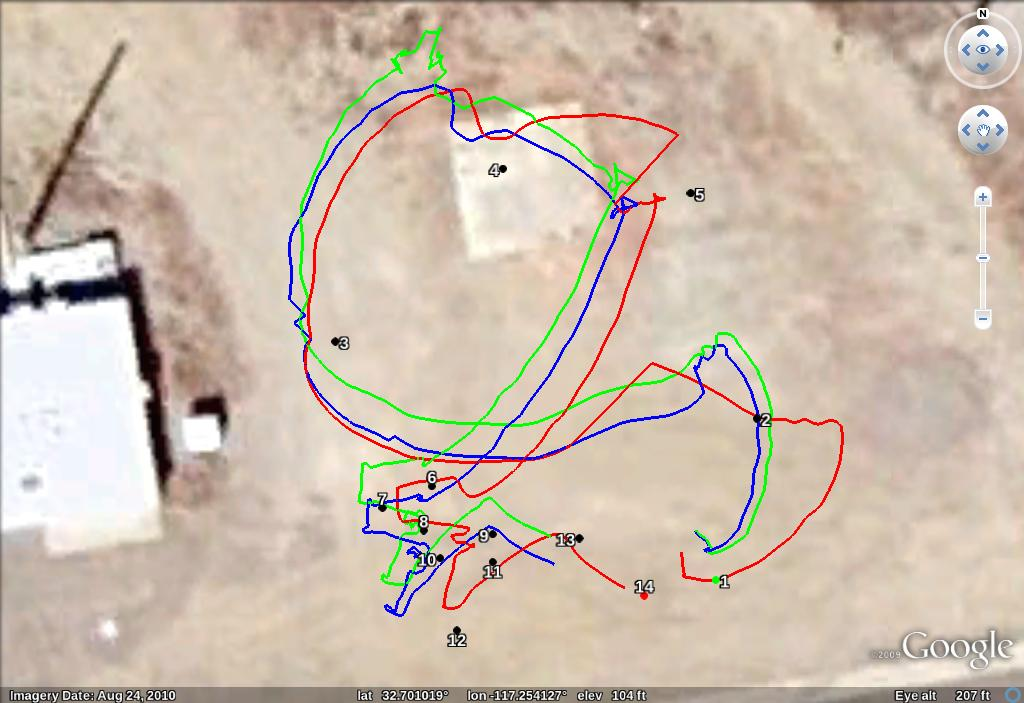
\includegraphics[width=.75\textwidth]{images/GE/20101203_1551_kf_lyapOrigQR}
	\caption{Model Based Controller with Original Noise Models}
	\label{fig:kfResults1}
\end{figure}

Running the model based controller with learned noise models resulted in the positions shown in Figure \ref{fig:kfResults2}. Here it can be seen that the Kalman filter position estimate is much closer to the GPS measurements for the entire route and that in certain places, such as near waypoint $4$ and between waypoint $6$ and waypoint $7$ the Kalman filter is able to remove discontinuities in the GPS position. Also, in the section of the route with waypoints close to each other to simulate navigation around obstacles the model based controller is able to drive through the waypoints.

\begin{figure}[ht!]
	\centering
	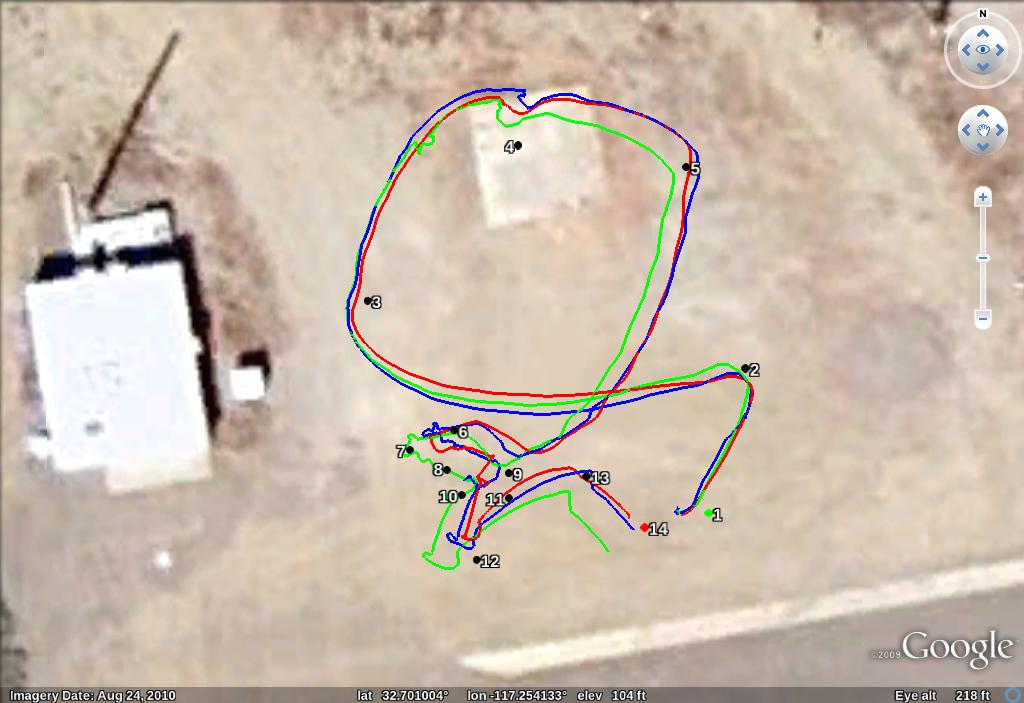
\includegraphics[width=.75\textwidth]{images/GE/20101203_1545_kf_lyapNewQR}
	\caption{Model Based Controller with Learned Noise Models}
	\label{fig:kfResults2}
\end{figure}

The PID controller with original noise models is shown in Figure \ref{fig:kfResults3}. Similar results are seen in regards to the Kalman filter position estimate snapping to the GPS measurements when significant divergence occurs between wayoint $2$ and waypoint $3$. The PID controller has trouble in the section of the route between waypoint $6$ and waypoint $12$ where the waypoints were set up close together to simulate obstacle along the route. In this section of the route the Kalman filter yaw estimate becomes very poor as the robot was driving in circles trying to reach the waypoints and as a result the Kalman filter position estimate diverges and would have snapped back to the GPS measurement if the route were not finished at waypoint $14$.

\begin{figure}[ht!]
	\centering
	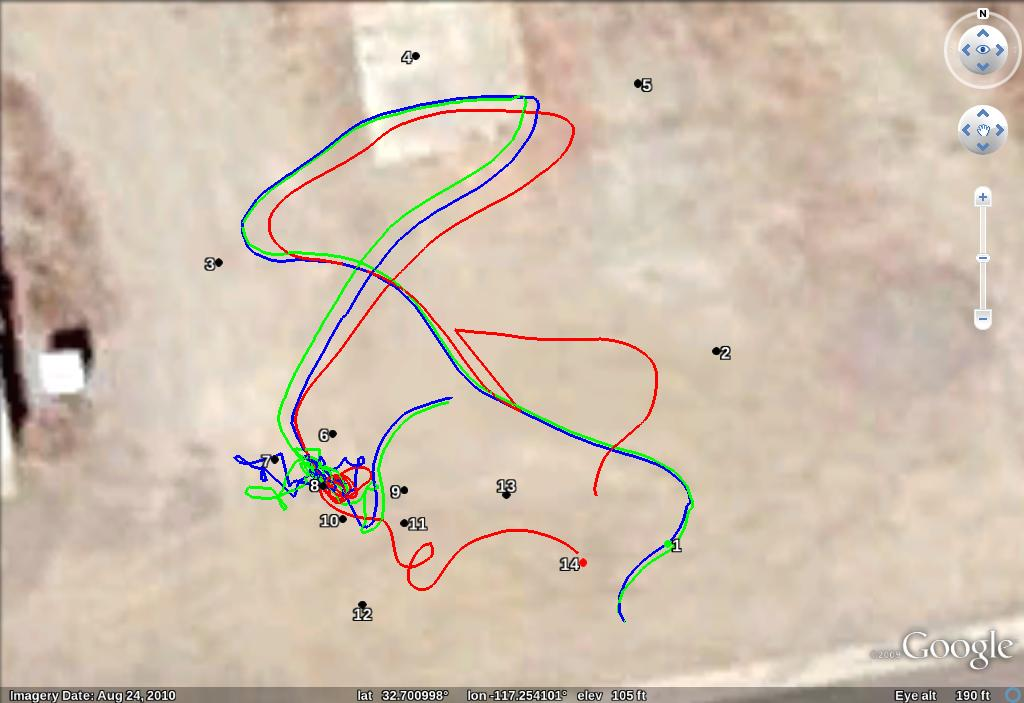
\includegraphics[width=.75\textwidth]{images/GE/20101203_1755_kf_pidOrigQR}
	\caption{PID Controller with Original Noise Models}
	\label{fig:kfResults3}
\end{figure}

The PID controller with learned noise models has similar trouble navigating the waypoints that are close together as seen in Figure \ref{fig:kfResults4}. However, with the learned noise models the Kalman filter position estimate stays much closer to the GPS measurements even when the robot is driving in circles. The improved position estimate is also indicative of an improved yaw estimate from the Kalman filter.

\begin{figure}[ht!]
	\centering
	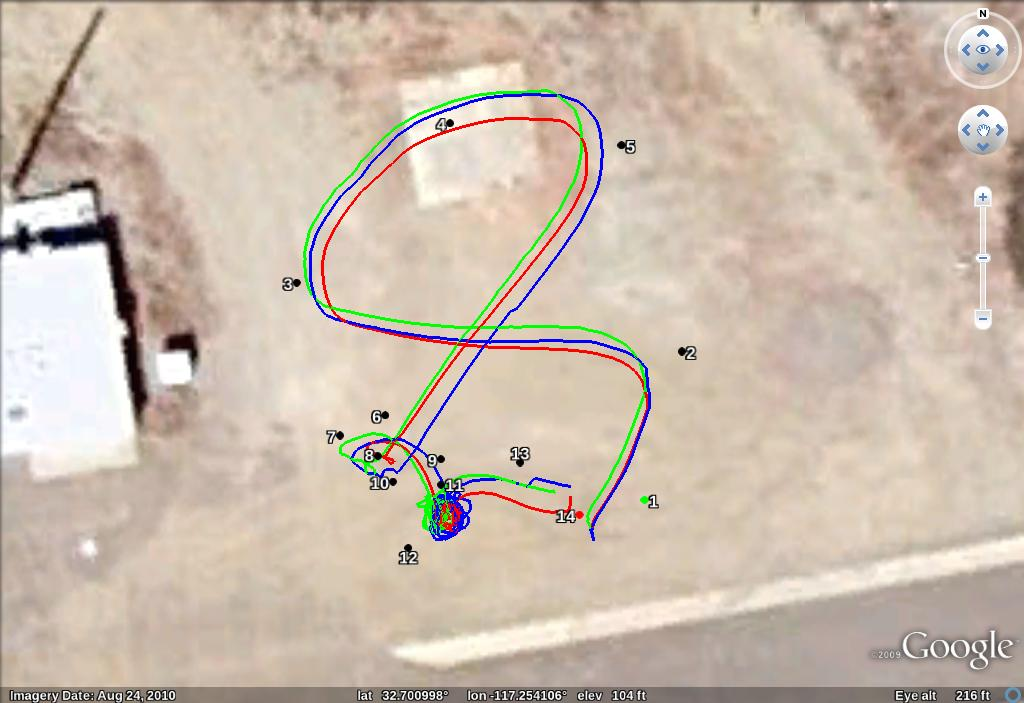
\includegraphics[width=.75\textwidth]{images/GE/20101203_1751_kf_pidNewQR}
	\caption{PID Controller with Learned Noise Models}
	\label{fig:kfResults4}
\end{figure}

\section{Model Based Controller Results}
\label{sec:lyapunovResults}
The linear and angular velocity outputs that were the result of running a simple route with the PID controller are shown in Figure \ref{fig:pidOutput}. This compares to the outputs of the model based controller shown in Figure \ref{fig:mbOutput} where it can be seen that the angular velocity is smooth and the linear velocity drives much faster, using $100\%$ effort at times but smoothly decelerating as waypoints are reached. The linear velocity output does not go to zero until the final waypoint is reached as a consequence of the moving target frame described in Chapter \ref{sec:drivingMode}. The errors for the model based controller are shown in Figure \ref{fig:mbErrors} which shows that $e$, $\alpha$ and $\theta$ decrease linearly at the rate given by the gain $\gamma$ and the eigenvalues of the matrix $A$ composed of the gains $h$ and $k$.

\begin{figure}[ht!]
	\centering
	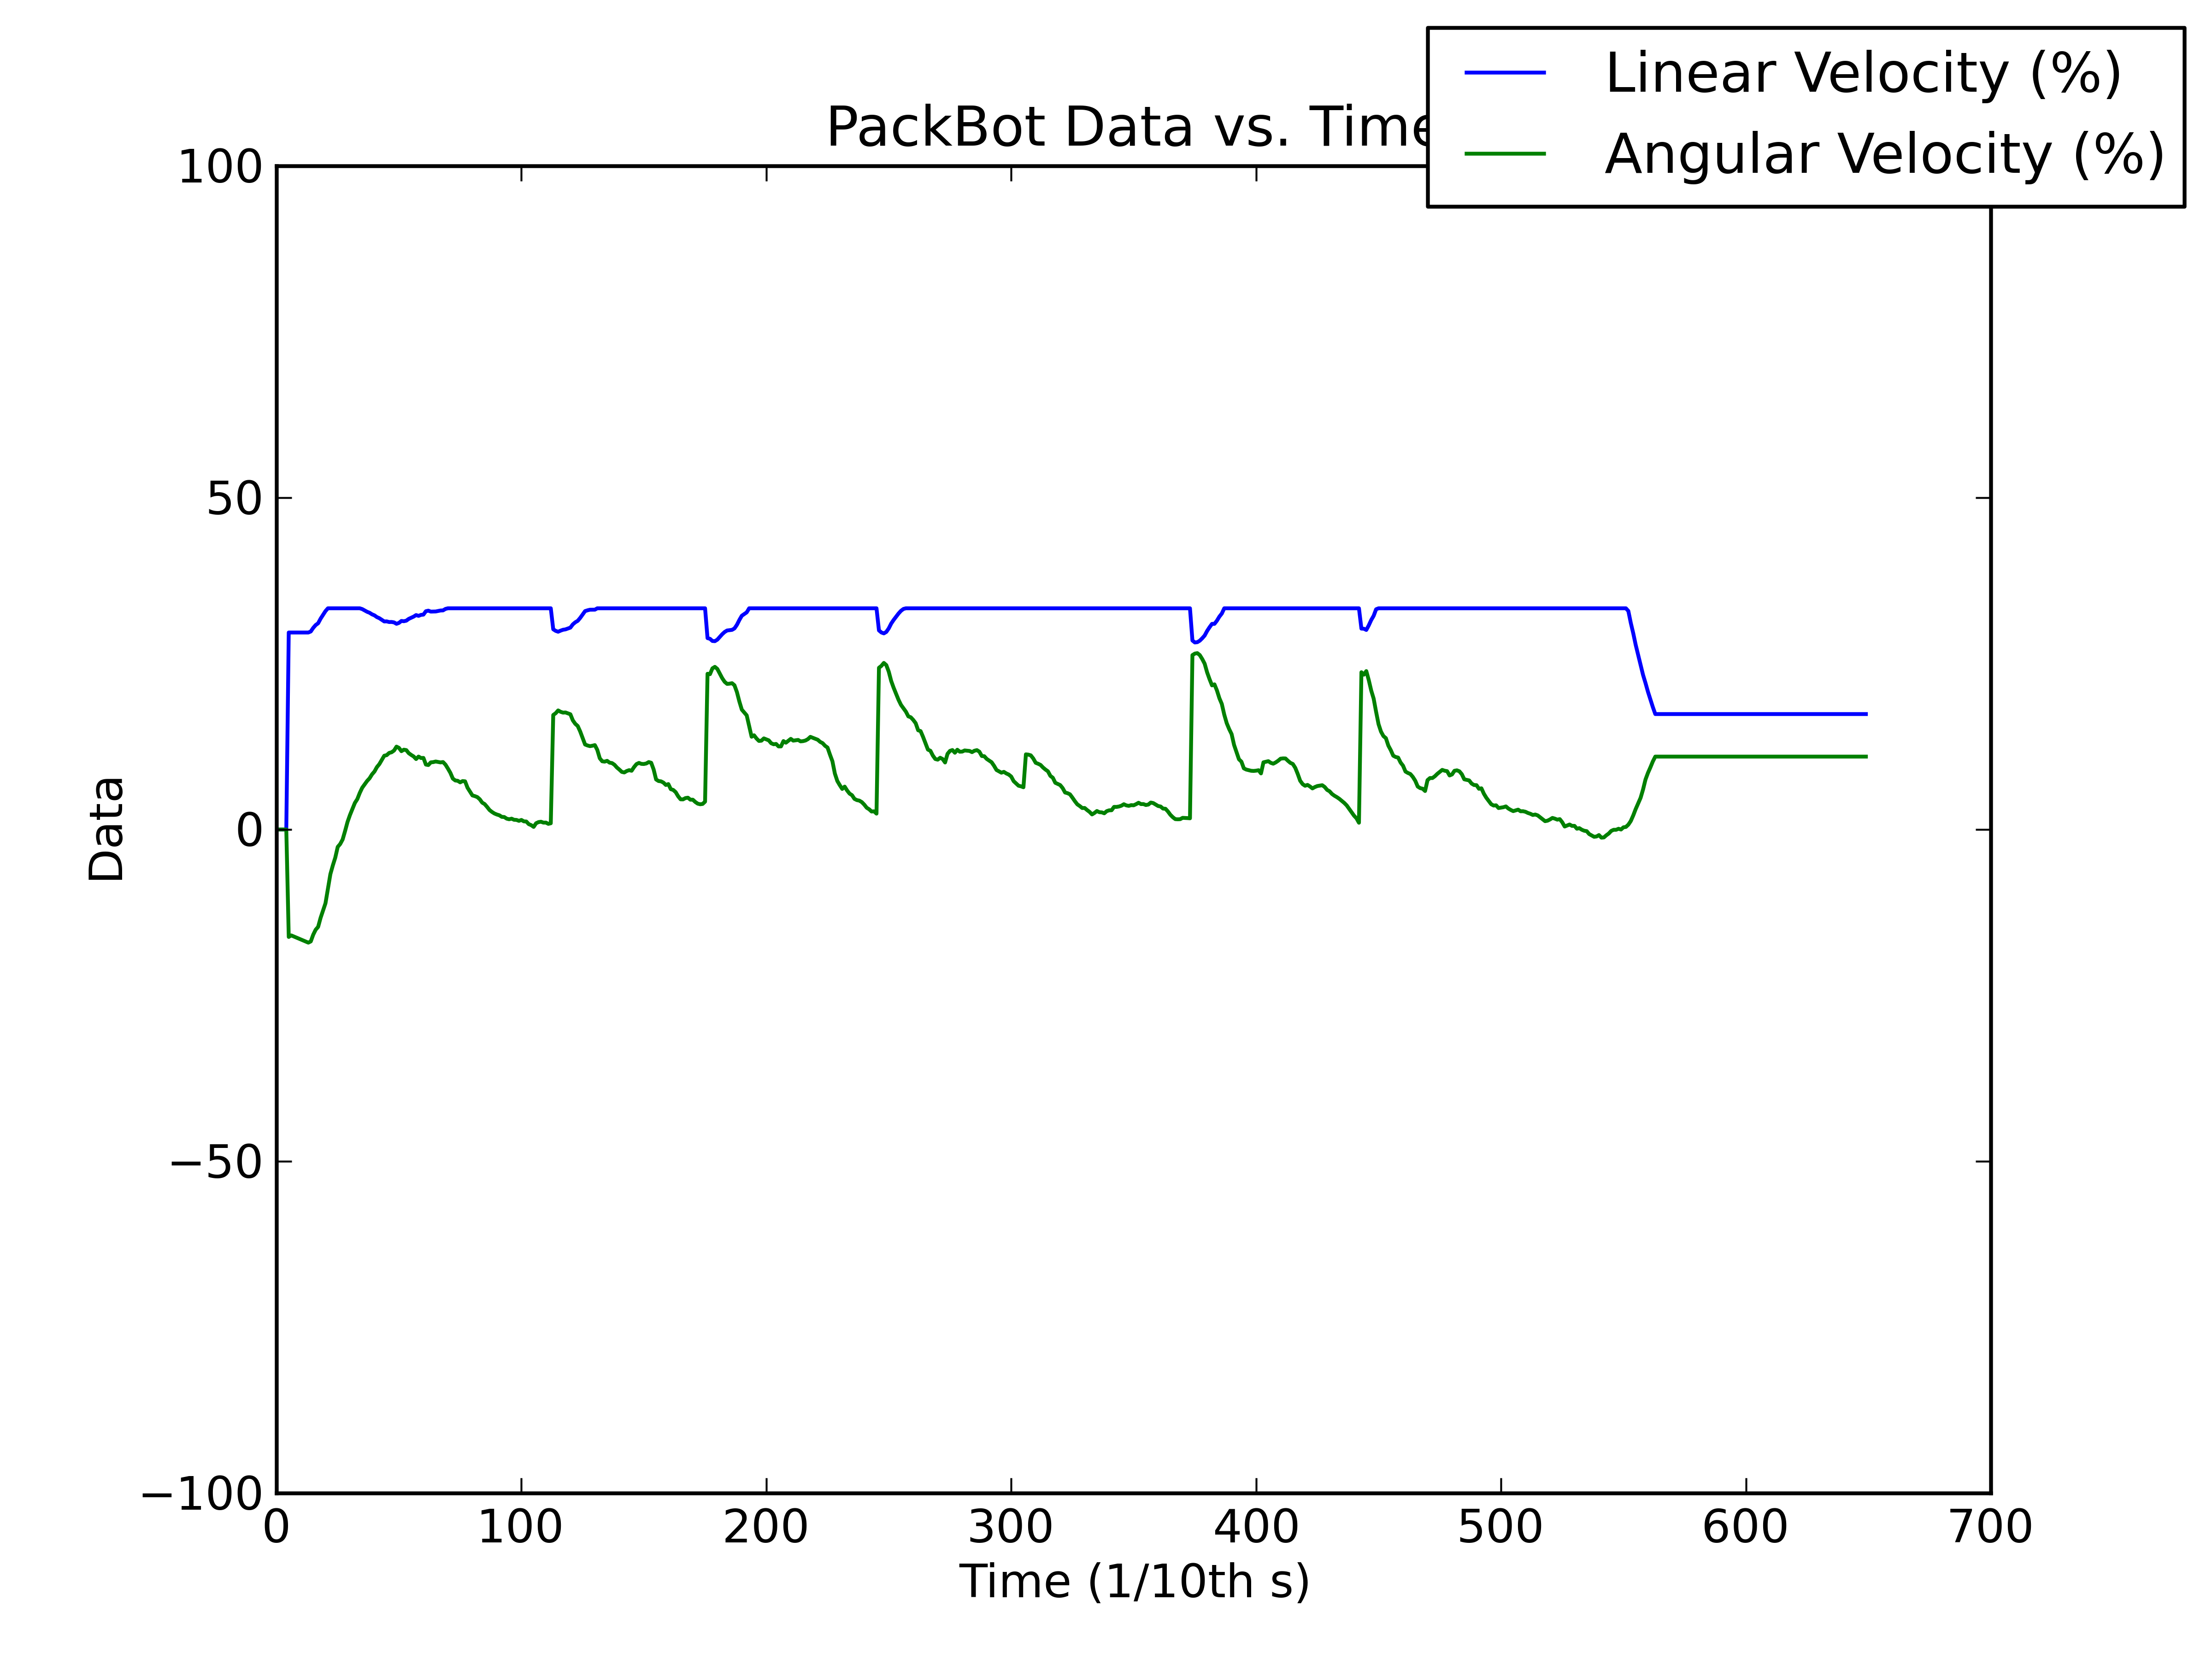
\includegraphics[width=.5\textwidth]{images/pbtx/20110109_1815_pbtx_simpleDrivePID}
	\caption{Typical PID Controller Velocity Output}
	\label{fig:pidOutput}
\end{figure}

\begin{figure}[ht!]
	\centering
	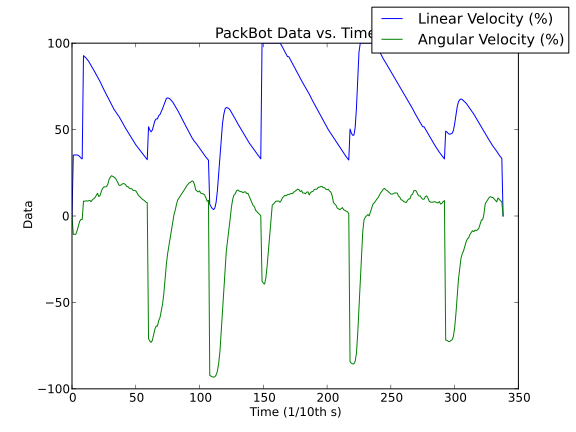
\includegraphics[width=.5\textwidth]{images/pbtx/20110113_1451_pbtx_simpleDrive}
	\caption{Typical Model Based Controller Velocity Output}
	\label{fig:mbOutput}
\end{figure}

\begin{figure}[ht!]
	\centering
	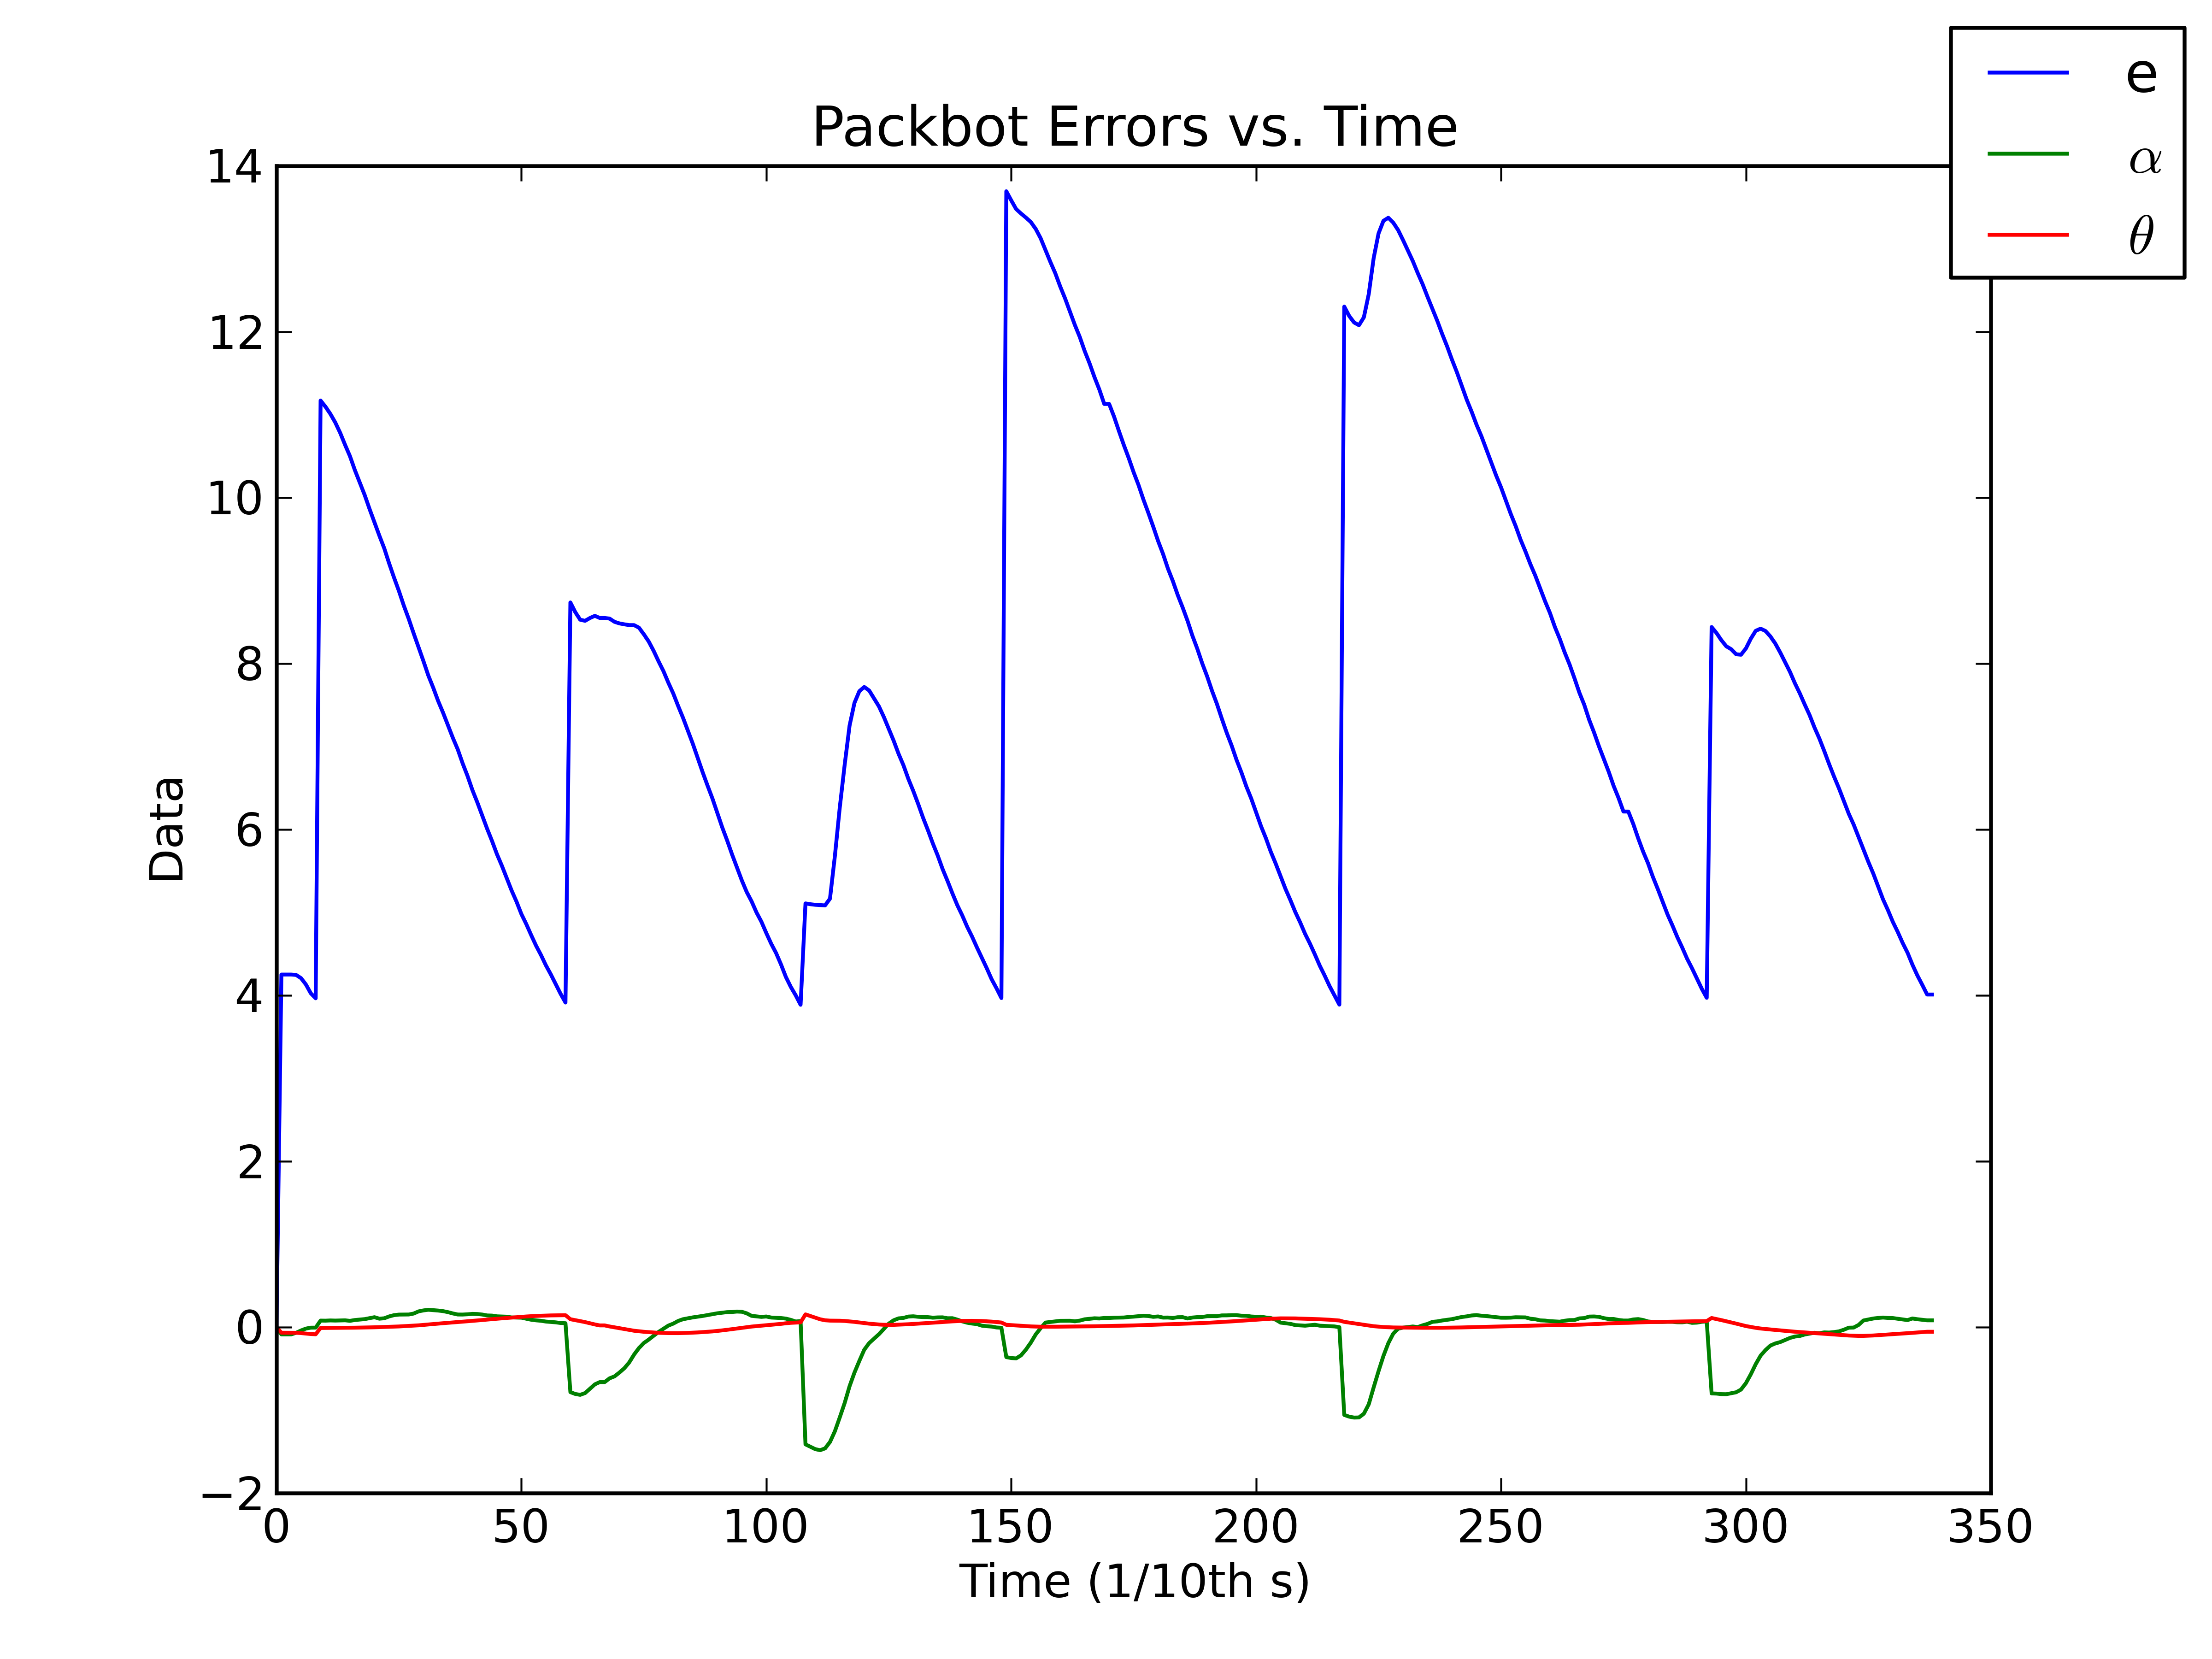
\includegraphics[width=.5\textwidth]{images/pbtx/20110113_1451_pbtx_simpleDriveErrors}
	\caption{Model Based Controller Errors}
	\label{fig:mbErrors}
\end{figure}

\subsection{Controller Comparison}
\label{sec:controllerComparison}
For both PID (Chapter \ref{sec:pid}, Table \ref{tab:PIDGainEffects}) and the model based controller (Chapter \ref{sec:lyapunovTrajectoryConvergence}) gains have to be selected, the difference being that stability is the goal when selecting PID gains whereas stability is guaranteed with the model based controller. More advanced behaviors such as three point turns are a consequence of the control law in (\ref{eq:lyapunovControlLaw}) derived using a kinematic model of the robot. The other very large difference between the controllers is that a table of gains must be tuned for the PID controller to work at varying linear velocities but the model based controller works very well at different linear and angular velocities. Also, when properties of the robot such as mass are changed by using different payloads for the system the entire table of PID gains must be retuned while, at most, one set of gains must be retuned for the model based controller. This last benefit of the model based controller makes it very appealing to use in fielded systems since it reduces the amount of maintenance and effort required to keep the robot in optimal working condition. The model based controller will also allow for improved navigation performance near obstacles which leads directly to improved autonomy for the robot. The local path planner is much simpler with the model based controller since it simply requires moving the target frame based on the calculated errors whereas the PID controller uses an entirely new algorithm that is not a normal part of the control algorithm to set the carrot following mode \cite{Hogg02}.

Many different controller configurations are possible based on varying the gains used and the calculation of the desired heading at waypoints. The tested configurations are shown in Table \ref{tab:resultsControllersSetup}.

\begin{table}[ht!]
\caption{Controller Setups}
\small
\centering
\begin{tabular}{@{}lllllr@{}} \toprule
Setup & Controller  & $\gamma$ & $h$  & $k$               & $\theta^\star$ \\ \midrule
1     & PID         & N/A      & N/A  & N/A               & N/A \\
2     & Fuzzy Logic & N/A      & N/A  & N/A               & N/A \\
3     & Model Based & 0.25     & 0.33 & 0.30              & CN \\
4     & Model Based & 0.25     & 0.33 & 0.30              & PC \\
5     & Model Based & 0.25     & 1.10 & $2\gamma\sqrt{h}$ & CN \\
6     & Model Based & 0.25     & 1.10 & $2\gamma\sqrt{h}$ & PC \\ \bottomrule
\end{tabular}
\label{tab:resultsControllersSetup}
\end{table}

Note that in all cases for the model based controller the desired goal heading $\theta^\star$ for the final waypoint was set to be the angle from the previous waypoint to the last waypoint.

Each controller configuration was run on several courses that test specific behaviors.
\begin{itemize}
\item Allowing for maximum velocities to be sustained with large amounts of open space on the route by having long path segments shown in Figure \ref{fig:routeLong}. This route used $\lambda = 0.001$, $\epsilon = 2.0$, $R_{\text{cap}} = 1.0$. There are $13$ waypoints covering a total of $90.73 m$ with an average distance between them of $7.56 m$.
\begin{figure}[ht!]
	\centering
	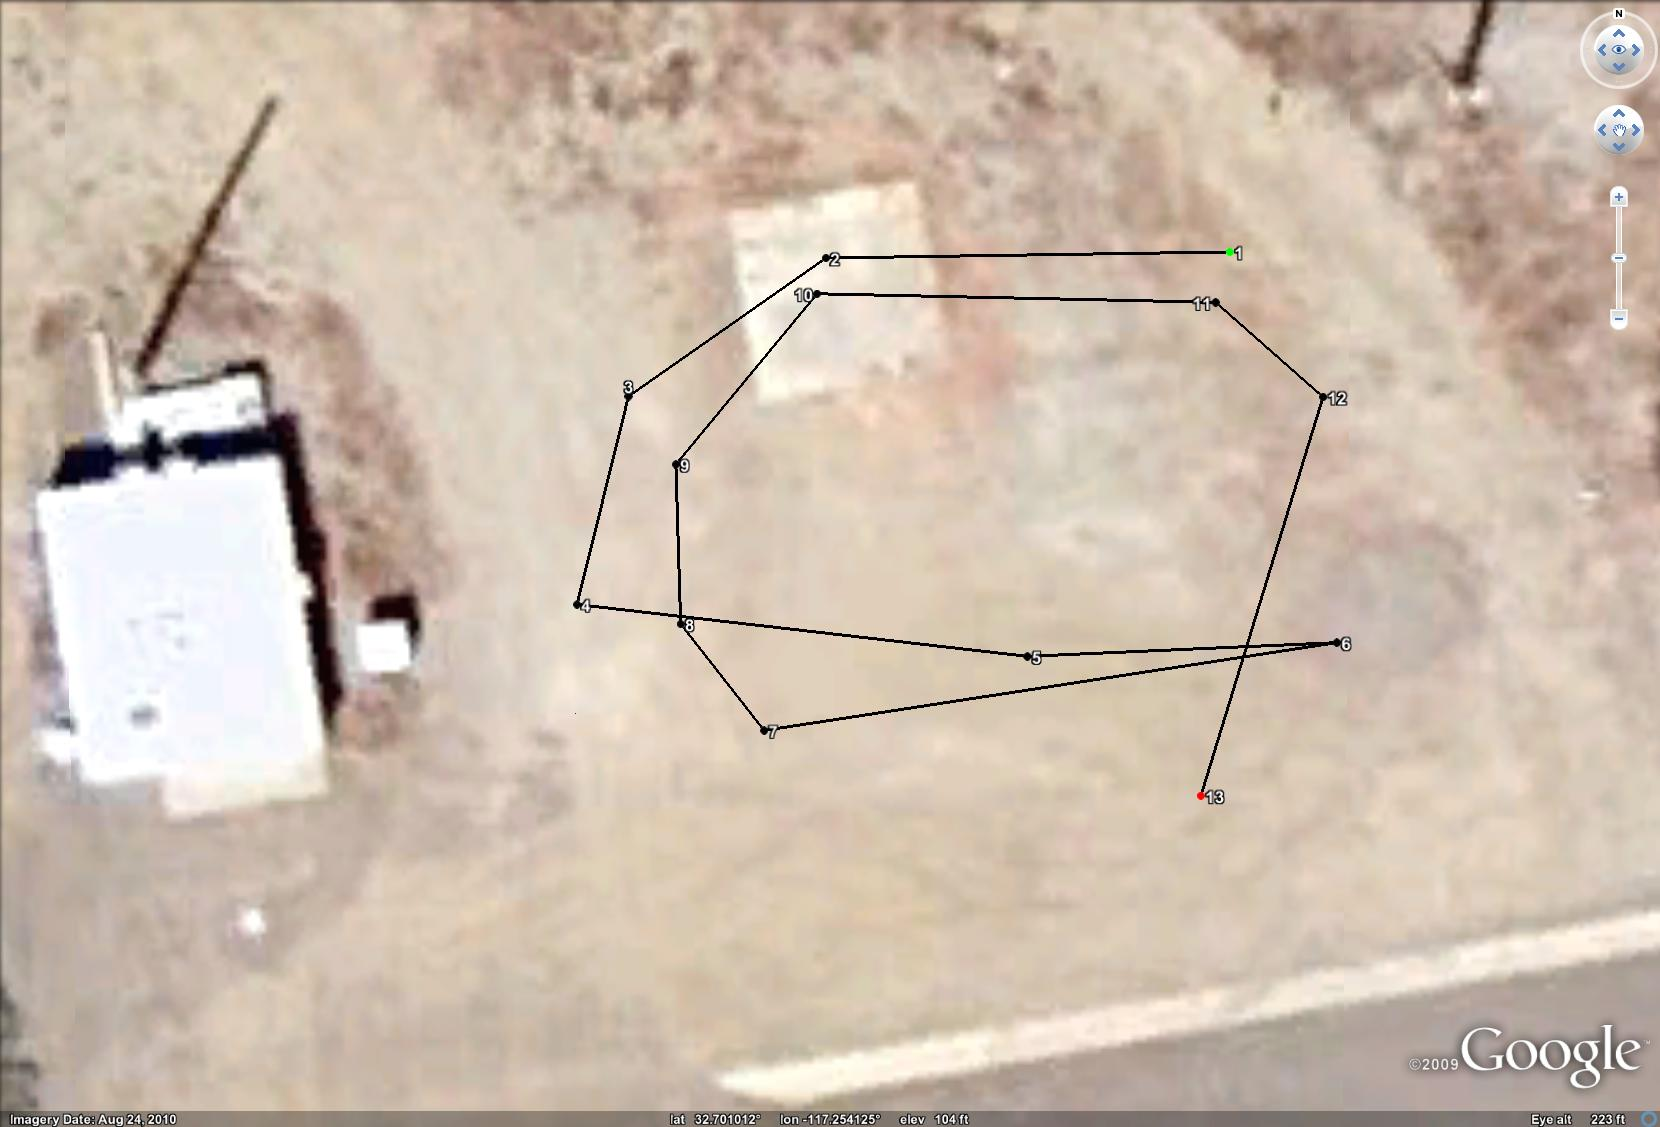
\includegraphics[width=.5\textwidth]{images/GE/GELongSegmentsRoute2}
	\caption{Route with Long Path Segments}
	\label{fig:routeLong}
\end{figure}
\item Short path segments between waypoints to simulate obstacles along the route shown in Figure \ref{fig:routeShort}. This route used $\lambda = 0.001$, $\epsilon = 1.0$, $R_{\text{cap}} = 0.2$. There are $27$ waypoints covering a total of $43.18 m$ with an average distance between them of $1.66 m$.
\begin{figure}[ht!]
	\centering
	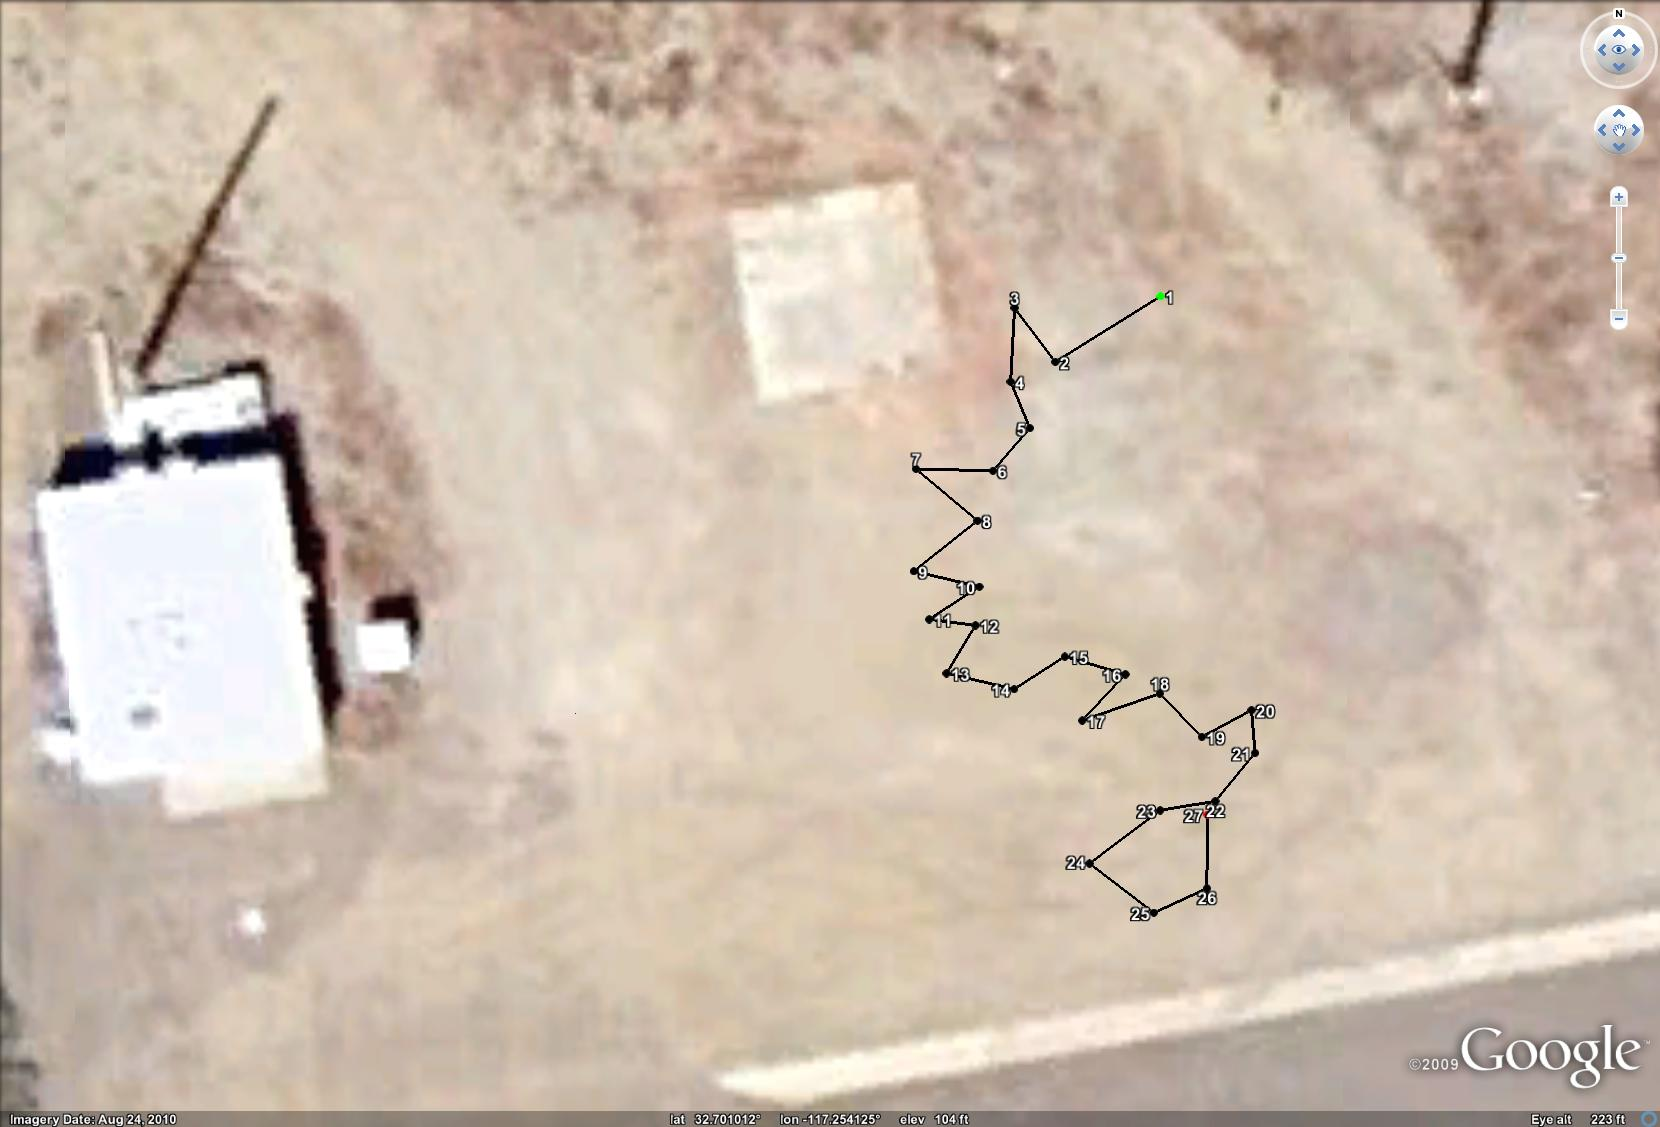
\includegraphics[width=.5\textwidth]{images/GE/GEShortSegmentsRoute2}
	\caption{Route with Short Path Segments}
	\label{fig:routeShort}
\end{figure}
\item A mixture of long and short path segments shown in Figure \ref{fig:routeMixed}. This route used $\lambda = 0.001$, $\epsilon = 1.5$, $R_{\text{cap}} = 0.5$. There are $13$ covering a total of $70.87 m$ waypoints with an average distance between them of $5.45 m$.
\begin{figure}[ht!]
	\centering
	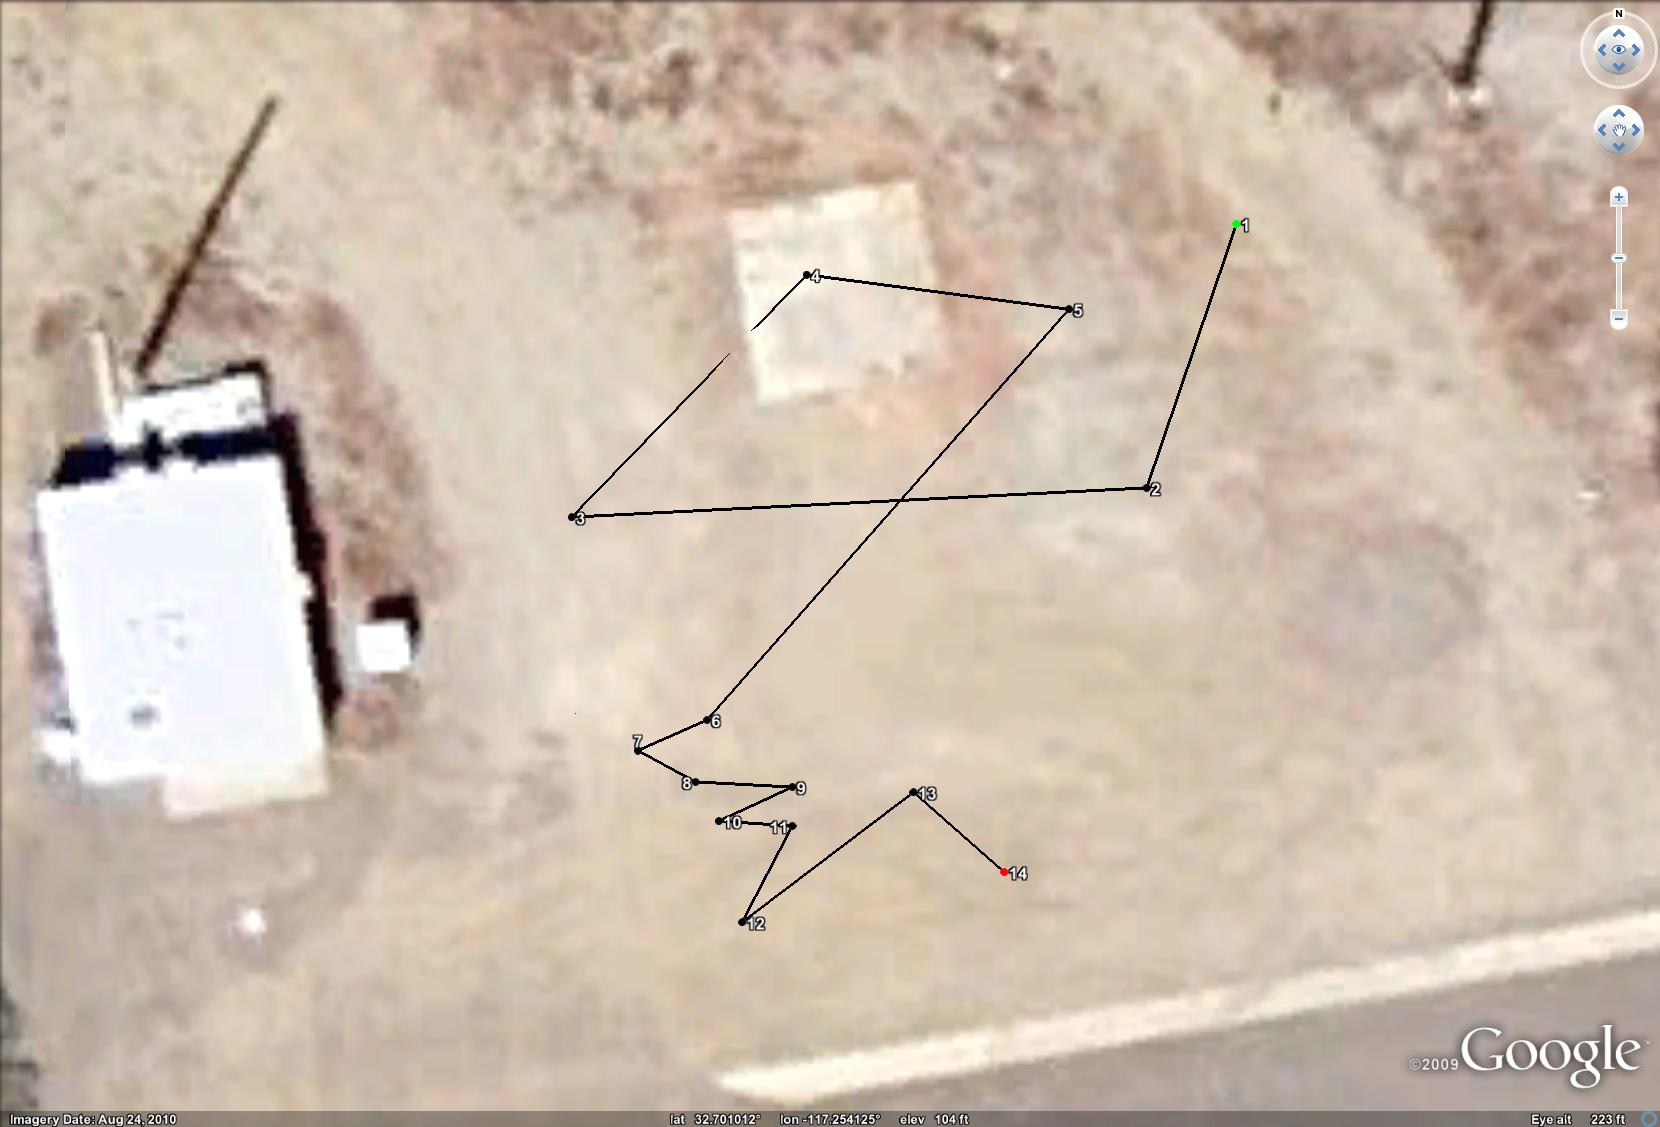
\includegraphics[width=.5\textwidth]{images/GE/GEMixedSegmentsRoute2}
	\caption{Route with Mixed Length Path Segments}
	\label{fig:routeMixed}
\end{figure}
\end{itemize}
The variable $R_{\text{cap}}$ is the capture radius for each waypoint which is used to determine when the robot is close enough to the current waypoint that the next waypoint should be set as the current target.

The results using the different setups described are shown for the different routes in Tables \ref{tab:resultsControllersOpenSpace} - \ref{tab:resultsControllersMixed} where the metrics used to compare the controller performance are
\begin{itemize}
\item the time required to complete the course,
\item the average cross track (XT) error during the course to show whether the robot followed a straight line between waypoints which is important when obstacles are in the area and not important when large amounts of open space are available for navigation (although some operators become nervous when the robot trajectory has large curvature and deviates from a straight line path even if open space is available),
\item the maximum velocity achieved by the robot during the course,
\item the number of times that the robot stops where a stop is defined as the robot having a velocity that drops below a small velocity,
\item the average error in heading from the desired heading when reaching the waypoints which is not available for the PID or fuzzy logic controllers but does help to differentiate between the model based controllers that have different goal headings and gains,
\item the total effort used by summing the values of linear and angular velocity over an entire run but does not take into account accelerations or the orientation of the robot.
\end{itemize}
For the model based controller in parking mode the same algorithm was run but $\epsilon=0$ was enough to keep the distance error from increasing and $\lambda$ was unused.

\begin{table}[ht!]
\caption{Controller Comparison on Open Space Route}
\small
\centering
\begin{tabular}{@{}llllr@{}} \toprule
Setup & Time (s) & XT (m) & $u_{\text{max}}$ (\%) & Stops \\ \midrule
1     & 82.67    & 0.61   & 33.3                  & 1     \\
2     & 0        & 0      & 0                     & 0     \\
3     & 75.12    & 2.52   & 100.0                 & 3     \\
4     & 71.42    & 2.71   & 100.0                 & 4     \\
5     & 110.09   & 2.42   & 100.0                 & 14    \\
6     & 75.45    & 2.80   & 100.0                 & 5     \\ \bottomrule
\end{tabular}
\label{tab:resultsControllersOpenSpace}
\end{table}

\begin{table}[ht!]
\caption{Controller Comparison on Simulated Obstacle Route}
\small
\centering
\begin{tabular}{@{}llllr@{}} \toprule
Setup & Time (s) & XT (m) & $u_{\text{max}}$ (\%) & Stops \\ \midrule
1     & N/A      & N/A    & N/A                   & N/A   \\
2     & 0        & 0      & 0                     & 0     \\
3     & 134.92   & 0.85   & 42.52                 & 20    \\
4     & 75.92    & 0.94   & 50.86                 & 21    \\
5     & 232.09   & 0.79   & 27.90                 & 31    \\
6     & 75.99    & 0.91   & 49.96                 & 23    \\ \bottomrule
\end{tabular}
\label{tab:resultsControllersObstacles}
\end{table}

\begin{table}[ht!]
\caption{Controller Comparison on Mixed Route}
\small
\centering
\begin{tabular}{@{}llllr@{}} \toprule
Setup & Time (s) & XT (m) & $u_{\text{max}}$ (\%) & Stops \\ \midrule
1     & N/A      & N/A    & N/A                   & N/A   \\
2     & 0        & 0      & 0                     & 0     \\
3     & 103.39   & 2.51   & 100.0                 & 11    \\
4     & 76.91    & 2.98   & 100.0                 & 12    \\
5     & 164.65   & 2.34   & 100.0                 & 22    \\
6     & 83.84    & 2.87   & 100.0                 & 12    \\ \bottomrule
\end{tabular}
\label{tab:resultsControllersMixed}
\end{table}

The PID controller only worked well on the route with long path segments. For the short and mixed path segment routes it actually became sad to watch and the tests were aborted because the robot was just spinning in circles and running the batteries down, similar to what was seen in Figure \ref{fig:kfResults4}.

All of the model based controllers are fairly similar. However, it can be seen that Setup $3$ consistently has longer run times but smaller cross track errors. This indicates that during those runs the robot was on the line between the previous and current waypoints with a heading towards the waypoint but that the robot slowed down at each of the waypoints because the angle errors were larger than in other runs. For all three routes each configuration of the model based controller exhibits an inverse relationship between cross track error and time taken to complete the route. The best setup for the most common scenarios that SSCPAC robots will encounter is likely to be either Setup $4$ or Setup $6$ where the robot drives fast and stays fairly close the straight line path between waypoints. Those two setups have the desired goal heading, $\theta^\star$, set to be the angle from the previous waypoint to the current waypoint which has more to do with the robot staying on the line between waypoints than do the gains.
